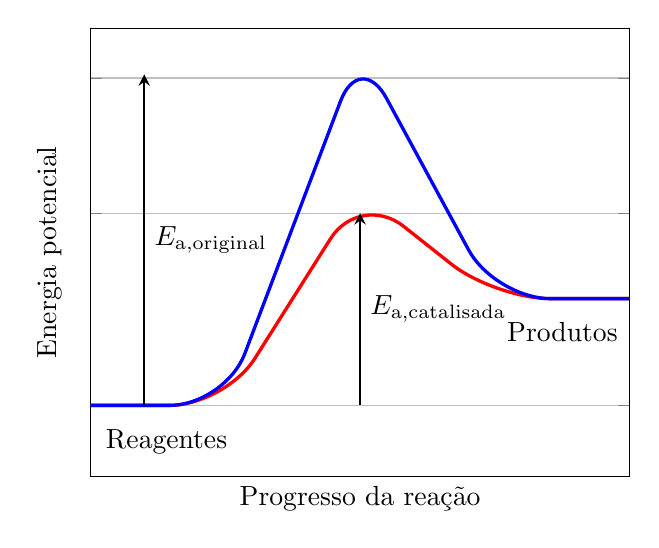
\begin{tikzpicture}
    \begin{axis}
        [
            grid = major,
            ylabel = {Energia potencial},
            xlabel = {Progresso da reação},
            xmin = 0, xmax = 4,
            ymin = -1, ymax = 5.3,
            xtick = \empty,
            ytick = {0, 2.70, 4.60},
            yticklabels = {},
        ]
        
        \draw [draw=red, very thick, rounded corners=2em]
            (axis cs: 0, 0) -- 
            (axis cs: 1, 0) -- 
            (axis cs: 2, 3) -- 
            (axis cs: 3, 1.5) --
            (axis cs: 4, 1.5);

        \draw [draw=blue, very thick, rounded corners=2em]
            (axis cs: 0, 0) -- 
            (axis cs: 1, 0) -- 
            (axis cs: 2, 5) -- 
            (axis cs: 3, 1.5) --
            (axis cs: 4, 1.5);
            
        \draw [ draw=black, thick, -stealth ]
            (axis cs: 0.4, 0.0) -- node [right] {$E_\mathrm{a, original}$}
            (axis cs: 0.4, 4.65);

        \draw [ draw=black, thick, -stealth ]
            (axis cs: 2.0, 0.0) -- node [right] {$E_\mathrm{a, catalisada}$}
            (axis cs: 2.0, 2.7);
        
        \node [ below, align=center ] at (axis cs:3.5,1.3) 
            { Produtos};

        \node [ below, align=center ] at (axis cs:0.6,-0.2) 
            { Reagentes  };

     \end{axis}
 \end{tikzpicture}